\chapter{Orbitales atómicos: formas, energías y tamaños}\label{ch:b2:atomic-orbitals}

Un átomo de hidrógeno no tiene borde: su electrón puede encontrarse a cualquier distancia del
núcleo, con una probabilidad que disminuye deprisa pero nunca llega a
cero. Sin embargo, los átomos tienen tamaño, y un átomo de sodio es casi el doble de ancho que un
átomo de cloro, aunque tiene menos electrones. El volumen del primer año designó los
estados de un electrón con tres números cuánticos; aquí cada uno de ellos se convierte en una
función de la posición, con una forma, nodos, signos y un tamaño, y un sencillo conjunto
de reglas los convierte en \omterm{def:b2:atomic-orbitals:orbital-energy}{energías orbitales} para cualquier átomo. Estas formas y estos signos
son lo que los cuatro capítulos siguientes combinan en orbitales moleculares.

\begin{recall}
El volumen del primer año: números cuánticos $n$, $l$, $m_l$, $m_s$; los orbitales atómicos como
estados $(n, l, m_l)$; capas y subcapas; efecto pantalla y carga nuclear
efectiva (de forma cualitativa); configuraciones electrónicas; los niveles del hidrógeno,
$-E_R/n^2$ con $E_R = \qty{13.6}{eV}$. De la física: la \omterm{def:b2:atomic-orbitals:wavefunction}{función de onda}, cuyo
módulo al cuadrado es una \omterm{def:b2:atomic-orbitals:wavefunction}{densidad de probabilidad}.
\end{recall}

\section{Las funciones de onda del átomo de hidrógeno}

\begin{definition}[Función de onda]\label{def:b2:atomic-orbitals:wavefunction}
El estado de un electrón se describe mediante una \emph{función de onda}\index{funcion de onda@función de onda}
$\psi(x, y, z)$; $|\psi|^2$ es su \emph{densidad de probabilidad}\index{densidad de probabilidad}:
la probabilidad de encontrar el electrón en un pequeño volumen $dV$ alrededor de
un punto es $|\psi|^2\,dV$, y $\int|\psi|^2\,dV = 1$ sobre todo el espacio (la función
está normalizada). Un orbital atómico es la función de onda de un electrón en un
átomo.
\end{definition}

\begin{definition}[Partes radial y angular]\label{def:b2:atomic-orbitals:radial-angular}
En coordenadas esféricas $(r, \theta, \varphi)$ centradas en el núcleo, los orbitales de
un átomo hidrogenoide se factorizan como $\psi_{nlm}(r, \theta, \varphi) = R_{nl}(r)\,
Y_{lm}(\theta, \varphi)$: la \emph{parte radial}\index{parte radial} $R_{nl}$ depende
de $n$ y $l$, y la \emph{parte angular}\index{parte angular} $Y_{lm}$, solo de $l$ y
$m_l$.
\end{definition}

\begin{theorem}[Los orbitales hidrogenoides]\label{thm:b2:atomic-orbitals:hydrogen}
Para un átomo de un solo electrón de carga nuclear $Ze$, con $\rho = Zr/a_0$ y $a_0 =
\qty{52.9}{pm}$ el radio de Bohr, las \omterm{def:b2:atomic-orbitals:radial-angular}{partes radiales} para $n \leq 3$ son, en unidades de
$(Z/a_0)^{3/2}$:
\[
\begin{array}{ll}
  R_{1s} = 2\,\mathrm e^{-\rho} &
  R_{2s} = \dfrac{1}{2\sqrt2}\,(2 - \rho)\,\mathrm e^{-\rho/2} \\[2ex]
  R_{2p} = \dfrac{1}{2\sqrt6}\,\rho\,\mathrm e^{-\rho/2} &
  R_{3s} = \dfrac{2}{81\sqrt3}\,(27 - 18\rho + 2\rho^2)\,\mathrm e^{-\rho/3} \\[2ex]
  R_{3p} = \dfrac{4}{81\sqrt6}\,(6\rho - \rho^2)\,\mathrm e^{-\rho/3} &
  R_{3d} = \dfrac{4}{81\sqrt{30}}\,\rho^2\,\mathrm e^{-\rho/3}
\end{array}
\]
y las \omterm{def:b2:atomic-orbitals:radial-angular}{partes angulares} reales son $Y_s = 1/\sqrt{4\pi}$; $Y_{p_x}, Y_{p_y}, Y_{p_z} =
\sqrt{3/(4\pi)}\,(x, y, z)/r$; $Y_{d_{xy}} = \sqrt{15/(4\pi)}\,xy/r^2$ (y análogamente
$xz$, $yz$), $Y_{d_{x^2-y^2}} = \sqrt{15/(16\pi)}\,(x^2 - y^2)/r^2$, $Y_{d_{z^2}} =
\sqrt{5/(16\pi)}\,(3z^2 - r^2)/r^2$. Sus energías son $E_n = -Z^2E_R/n^2$.
% ledger: const:a0, const:RyhcEV
\end{theorem}

\admitted

Estas funciones son las soluciones de la ecuación de Schrödinger para un electrón
y un núcleo, que se obtienen en el volumen del tercer año. Las funciones $p$ y $d$ reales son
combinaciones de las complejas indexadas por $m_l$; apuntan a lo largo de los ejes y
son las que se usan para construir enlaces.

\begin{omfigure}
\begin{minipage}[t]{0.27\linewidth}\vspace{0pt}
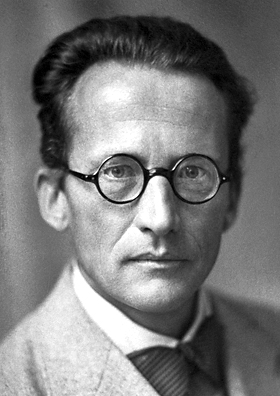
\includegraphics[width=\linewidth]{images/book3/schrodinger.jpg}
\end{minipage}\hfill
\begin{minipage}[t]{0.69\linewidth}\vspace{0pt}
{\small Erwin Schrödinger, que en 1926 escribió la ecuación de onda cuyas
soluciones para el átomo de hidrógeno son los orbitales de este capítulo, y recuperó
a partir de ellas los niveles de energía que Bohr había postulado. Compartió el Premio Nobel
de Física en 1933. (Fotografía: Fundación Nobel, dominio público,
Wikimedia Commons.)}
\end{minipage}
\end{omfigure}

\section{La parte radial}

La probabilidad de encontrar el electrón entre las esferas de radios $r$ y $r +
dr$ es $|\psi|^2$ integrada sobre la capa de volumen $4\pi r^2\,dr$; para cualquier
orbital, una vez integrados los ángulos, vale $r^2R^2\,dr$.

\begin{definition}[Distribución radial]\label{def:b2:atomic-orbitals:radial-distribution}
La \emph{función de distribución radial}\index{funcion de distribucion radial@función de distribución radial} de
un orbital es $P(r) = r^2R_{nl}(r)^2$: $P(r)\,dr$ es la probabilidad de que el
electrón esté entre $r$ y $r + dr$ del núcleo. El \emph{radio más
probable}\index{radio mas probable@radio más probable} es el valor de $r$ en su máximo más alto.
\end{definition}

\begin{proposition}[Normalización de 1s]\label{prop:b2:atomic-orbitals:normalised}
$\int_0^\infty P_{1s}(r)\,dr = 1$.
\end{proposition}

\begin{proof}
Con $Z = 1$ y $r$ en unidades de $a_0$, $P_{1s} = 4r^2\mathrm e^{-2r}$. Integrando dos veces por partes,
$\int_0^\infty r^2\mathrm e^{-2r}\,dr = \frac22\int_0^\infty r\,\mathrm e^{-2r}\,dr =
\frac12\int_0^\infty\mathrm e^{-2r}\,dr = \frac14$, y $4 \times \frac14 = 1$.
\end{proof}

\begin{proposition}[Radio más probable]\label{prop:b2:atomic-orbitals:most-probable}
Para el orbital 1s, el \omterm{def:b2:atomic-orbitals:radial-distribution}{radio más probable} es $a_0/Z$. Para un orbital con $l =
n - 1$ (1s, 2p, 3d, \dots), es $n^2a_0/Z$.
\end{proposition}

\begin{proof}
Para $l = n - 1$ la \omterm{def:b2:atomic-orbitals:radial-angular}{parte radial} no tiene nodo: $R \propto \rho^{n-1}\mathrm e^{-\rho/n}$,
luego $P \propto \rho^{2n}\mathrm e^{-2\rho/n}$ y $d\ln P/d\rho = 2n/\rho - 2/n$, nula
para $\rho = n^2$, es decir, $r = n^2a_0/Z$. Con $n = 1$, $r = a_0/Z$.
\end{proof}

\begin{proposition}[Radio medio de 1s]\label{prop:b2:atomic-orbitals:mean-radius}
La distancia media de un electrón 1s al núcleo es $\langle r\rangle = 3a_0/(2Z)$,
mayor que su \omterm{def:b2:atomic-orbitals:radial-distribution}{radio más probable}.
\end{proposition}

\begin{proof}
Con $Z = 1$: $\langle r\rangle = \int_0^\infty r\,P(r)\,dr = 4\int_0^\infty r^3\mathrm e^{-2r}
\,dr = 4 \times 3!/2^4 = 3/2$. La distribución tiene una larga cola a $r$ grande,
que desplaza la media más allá del máximo.
\end{proof}

\begin{definition}[Nodos]\label{def:b2:atomic-orbitals:node}
Una \emph{superficie nodal}\index{superficie nodal} de un orbital es una superficie sobre la que
la \omterm{def:b2:atomic-orbitals:wavefunction}{función de onda} se anula y cambia de signo. Es un \emph{nodo radial}\index{nodo radial}
(una esfera) cuando se anula la \omterm{def:b2:atomic-orbitals:radial-angular}{parte radial}, y un \emph{nodo
angular}\index{nodo angular} (un plano o un cono que pasa por el núcleo) cuando se anula la \omterm{def:b2:atomic-orbitals:radial-angular}{parte angular}.
\end{definition}

\begin{proposition}[Recuento de nodos]\label{prop:b2:atomic-orbitals:nodes}
Un orbital $(n, l)$ tiene $n - l - 1$ \omterm{def:b2:atomic-orbitals:node}{nodos radiales} y $l$ \omterm{def:b2:atomic-orbitals:node}{nodos angulares}, $n - 1$ en
total.
\end{proposition}

\begin{proof}
En las funciones del \cref{thm:b2:atomic-orbitals:hydrogen}: $R_{2s}$ se anula en
$\rho = 2$, $R_{3s}$ en las dos raíces de $2\rho^2 - 18\rho + 27$ ($\rho = 1.90$ y $7.10$),
$R_{3p}$ en $\rho = 6$; $R_{1s}$, $R_{2p}$, $R_{3d}$ no se anulan. La \omterm{def:b2:atomic-orbitals:radial-angular}{parte angular}
de un orbital p se anula en un plano ($z = 0$ para $p_z$), y la de un orbital d, en dos
planos o, para $d_{z^2}$, en un cono. El caso general se admite.
\end{proof}

\begin{omfigure}
\begin{tikzpicture}
\begin{axis}[width=0.55\linewidth, height=6cm, xmin=0, xmax=24, ymin=0, ymax=0.58,
  axis x line=bottom, axis y line=left, xlabel={$r/a_0$}, ylabel={$P(r)$},
  tick label style={font=\small}, label style={font=\small}, title={\small distribuciones radiales, $Z = 1$}]
\addplot[omThm, thick] table[x=r, y=s1] {figdata/out/bachelor-2-atomic-orbitals-a.dat};
\addplot[omDef, thick] table[x=r, y=s2] {figdata/out/bachelor-2-atomic-orbitals-a.dat};
\addplot[omDef, thick, dashed] table[x=r, y=p2] {figdata/out/bachelor-2-atomic-orbitals-a.dat};
\addplot[omProp, thick] table[x=r, y=s3] {figdata/out/bachelor-2-atomic-orbitals-a.dat};
\addplot[omProp, thick, dashed] table[x=r, y=p3] {figdata/out/bachelor-2-atomic-orbitals-a.dat};
\addplot[omProp, thick, dotted] table[x=r, y=d3] {figdata/out/bachelor-2-atomic-orbitals-a.dat};
\node[font=\scriptsize, omThm, anchor=west] at (axis cs:1.4,0.53) {1s};
\node[font=\scriptsize, omDef, anchor=south] at (axis cs:4.0,0.215) {2p};
\node[font=\scriptsize, omDef, anchor=south west] at (axis cs:6.4,0.17) {2s};
\node[font=\scriptsize, omProp, anchor=south] at (axis cs:10.5,0.12) {3d};
\node[font=\scriptsize, omProp, anchor=west] at (axis cs:17,0.085) {3s, 3p};
\end{axis}
\end{tikzpicture}\hfill
\begin{tikzpicture}
\begin{axis}[width=0.42\linewidth, height=6cm, xmin=0, xmax=20, ymin=-0.12, ymax=0.75,
  axis x line=middle, axis y line=left, xlabel={$r/a_0$}, ylabel={$R$},
  tick label style={font=\small}, label style={font=\small}, title={\small partes radiales}]
\addplot[omDef, thick] table[x=r, y=R2s] {figdata/out/bachelor-2-atomic-orbitals-b.dat};
\addplot[omProp, thick] table[x=r, y=R3s] {figdata/out/bachelor-2-atomic-orbitals-b.dat};
\node[font=\scriptsize, omDef, anchor=west] at (axis cs:0.4,0.62) {$R_{2s}$};
\node[font=\scriptsize, omProp, anchor=west] at (axis cs:0.6,0.30) {$R_{3s}$};
\node[font=\scriptsize, anchor=south west] at (axis cs:3,0.15) {nodo};
\draw[thin, ->] (axis cs:3,0.15) -- (axis cs:2.05,0.01);
\end{axis}
\end{tikzpicture}

{\small A la izquierda: distribuciones radiales $P(r) = r^2R^2$ de los orbitales del hidrógeno hasta
$n = 3$; cuanto mayor es $n$, más lejos está el electrón, y los orbitales s tienen
pequeños máximos interiores (penetración). A la derecha: $R_{2s}$ y $R_{3s}$ cambian de signo en sus
\omterm{def:b2:atomic-orbitals:node}{nodos radiales} ($r = 2a_0$; $1.90a_0$ y $7.10a_0$).}
\end{omfigure}

\begin{omfigure}
\begin{tikzpicture}
\begin{axis}[scale only axis, width=0.32\linewidth, height=0.32\linewidth,
  xmin=-6, xmax=6, ymin=-6, ymax=6, axis lines=none, title={\small 1s}]
\addplot[only marks, mark=*, mark size=0.25pt, omDef] table[x=x, y=y] {figdata/out/bachelor-2-atomic-orbitals-c-1s.dat};
\end{axis}
\end{tikzpicture}\hspace{0.12\linewidth}%
\begin{tikzpicture}
\begin{axis}[scale only axis, width=0.32\linewidth, height=0.32\linewidth,
  xmin=-14, xmax=14, ymin=-14, ymax=14, axis lines=none, title={\small 2s}]
\addplot[only marks, mark=*, mark size=0.25pt, omDef] table[x=x, y=y] {figdata/out/bachelor-2-atomic-orbitals-c-2s.dat};
\draw[densely dashed, omThm] (axis cs:0,0) circle[radius=2];
\end{axis}
\end{tikzpicture}

{\small Representaciones por densidad de puntos de los orbitales 1s y 2s del hidrógeno en un plano
que pasa por el núcleo: la densidad de puntos sigue $|\psi|^2$ (muestreo
determinista). La nube 2s tiene un anillo vacío, el \omterm{def:b2:atomic-orbitals:node}{nodo radial} en $2a_0$ (discontinuo);
los marcos tienen 12 y 28 $a_0$ de ancho.}
\end{omfigure}

\section{La parte angular}

La \omterm{def:b2:atomic-orbitals:radial-angular}{parte angular} fija la forma. Un orbital s es esférico; un orbital p tiene dos
lóbulos de signos opuestos a lo largo de su eje, separados por un plano nodal; un orbital d tiene
cuatro lóbulos de signos alternos (o, para $d_{z^2}$, dos lóbulos y un anillo). El signo
de un lóbulo no tiene significado físico por sí mismo ($\psi$ y $-\psi$ describen el mismo
estado), pero los signos relativos de dos orbitales deciden, en el capítulo siguiente,
si se combinan para formar un enlace.

\begin{omfigure}
\begin{tikzpicture}[font=\small]
  \pic at (0,0) {oms={1}};
  \node[below] at (0,-0.75) {s};
  \pic at (2.0,0) {omp={1}{0}};
  \draw[->, black!55, thin] (1.0,0) -- (3.0,0) node[right, font=\tiny] {$x$};
  \node[below] at (2.0,-0.75) {$\mathrm p_x$};
  \pic at (4.2,0) {omp={1}{90}};
  \draw[->, black!55, thin] (4.2,-0.95) -- (4.2,0.95) node[above, font=\tiny] {$z$};
  \node[below] at (4.75,-0.75) {$\mathrm p_z$};
  \pic at (6.6,0) {omdxy}; \node[below] at (6.6,-1.0) {$\mathrm d_{xy}$};
  \pic at (9.0,0) {omdx2y2}; \node[below] at (9.0,-1.0) {$\mathrm d_{x^2-y^2}$};
  \pic at (11.4,0) {omdz2}; \node[below] at (11.4,-1.0) {$\mathrm d_{z^2}$};
\end{tikzpicture}

{\small Orbitales atómicos reales, esquema: los lóbulos muestran las regiones en las que $|\psi|$
es grande, coloreadas según el signo de $\psi$ (azul positivo, naranja negativo). Los
orbitales $\mathrm d_{xz}$ y $\mathrm d_{yz}$ tienen la forma de $\mathrm d_{xy}$ en
los planos que indican sus nombres.}
\end{omfigure}

\begin{method}[Esbozar un orbital a partir de sus números cuánticos]\label{met:b2:atomic-orbitals:draw-orbital}
\begin{enumerate}
  \item A partir de $l$, la forma: s (esfera), p (dos lóbulos), d (cuatro lóbulos, o dos
        lóbulos y un anillo para $d_{z^2}$); a partir del subíndice, la orientación.
  \item Cuéntense los $l$ \omterm{def:b2:atomic-orbitals:node}{nodos angulares} (planos que pasan por el núcleo) y dense
        signos opuestos a los lóbulos adyacentes.
  \item Cuéntense los $n - l - 1$ \omterm{def:b2:atomic-orbitals:node}{nodos radiales}: capas internas de signo opuesto dentro
        de los lóbulos principales (normalmente omitidas en los esbozos).
  \item Escálese con $n^2a_0/Z$: mayor $n$, orbital más grande; mayor $Z$, más pequeño.
\end{enumerate}
\end{method}

\section{Átomos polielectrónicos}

En un átomo con varios electrones, cada electrón siente el núcleo apantallado por
los demás. Los orbitales conservan las formas de los del hidrógeno, con una carga
efectiva $Z^*$ en lugar de $Z$, y la energía de una subcapa depende ahora de $l$ además
de $n$: un electrón s, cuya distribución radial tiene máximos interiores cerca del
núcleo, está menos apantallado que un electrón p de la misma capa, y un p, menos
que un d.

\begin{definition}[Reglas de Slater]\label{def:b2:atomic-orbitals:slater}
Las \emph{reglas de Slater}\index{reglas de Slater} estiman la carga nuclear efectiva
$Z^* = Z - \sigma$ que siente un electrón. Los electrones se agrupan como
(1s) (2s, 2p) (3s, 3p) (3d) (4s, 4p) (4d) (4f) (5s, 5p) \dots; la constante de
apantallamiento $\sigma$ de un electrón es la suma de las contribuciones de los demás
electrones: 0.35 por cada otro electrón del mismo grupo (0.30 dentro de 1s);
para un electrón s o p, 0.85 por cada electrón de la capa $n - 1$ y 1.00 por
cada electrón de las capas inferiores; para un electrón d o f, 1.00 por cada electrón
de los grupos inferiores al suyo. Los grupos superiores no contribuyen.
\end{definition}

\begin{omfigure}
\small
\renewcommand{\arraystretch}{1.2}
\begin{tabular}{l|ccccc}
electrón estudiado & mismo grupo & capa $n - 1$ & capas inferiores & grupos superiores \\ \hline
1s & 0.30 & --- & --- & 0 \\
$n$s, $n$p & 0.35 & 0.85 & 1.00 & 0 \\
$n$d, $n$f & 0.35 & 1.00 & 1.00 & 0 \\
\end{tabular}

\smallskip
{\small Constantes de apantallamiento de Slater, por electrón apantallante. Los números
cuánticos principales efectivos son $n^* = 1, 2, 3, 3.7, 4.0, 4.2$ para $n = 1$ a 6.}
\end{omfigure}

\begin{method}[Calcular una carga efectiva]\label{met:b2:atomic-orbitals:slater}
\begin{enumerate}
  \item Escríbase la configuración en los grupos de Slater, por orden de $n$, con s y p
        juntos y d y f aparte.
  \item Elíjase el electrón; súmese 0.35 por cada otro electrón de su grupo.
  \item Súmese 0.85 (electrón s o p) o 1.00 (d o f) por cada electrón de la capa inmediatamente
        inferior, y 1.00 por cada electrón más profundo.
  \item $Z^* = Z - \sigma$.
\end{enumerate}
\end{method}

\begin{definition}[Energía y radio orbitales]\label{def:b2:atomic-orbitals:orbital-energy}
En el modelo de Slater, la \emph{energía orbital}\index{energia orbital@energía orbital} de un electrón
de carga efectiva $Z^*$ y número cuántico principal efectivo $n^*$ es
$\varepsilon = -E_RZ^{*2}/n^{*2}$, y su \emph{radio orbital}\index{radio orbital}
es $n^{*2}a_0/Z^*$, el \omterm{def:b2:atomic-orbitals:radial-distribution}{radio más probable} de un orbital hidrogenoide de carga
$Z^*$.
\end{definition}

\begin{proposition}[Energías de Slater]\label{prop:b2:atomic-orbitals:slater-energy}
La energía de un grupo de $k$ electrones de carga efectiva $Z^*$ es aproximadamente
$k\varepsilon = -kE_RZ^{*2}/n^{*2}$, y la energía electrónica total del átomo
es la suma sobre sus grupos.
\end{proposition}

\admitted

\begin{example}[El hierro: ¿4s o 3d primero?]\label{ex:b2:atomic-orbitals:iron}
El hierro es $[\ce{Ar}]\,3\mathrm d^6\,4\mathrm s^2$. Un electrón 4s: $\sigma = 0.35 + 14
\times 0.85 + 10 \times 1.00 = 22.25$, $Z^* = 3.75$, $\varepsilon = -13.6 \times
3.75^2/3.7^2 = \qty{-14.0}{eV}$. Un electrón 3d: $\sigma = 5 \times 0.35 + 18 \times 1.00 =
19.75$, $Z^* = 6.25$, $\varepsilon = -13.6 \times 6.25^2/9 = \qty{-59}{eV}$. Los electrones
3d están mucho más fuertemente ligados: aunque el 4s se llena primero en el
orden de llenado, es un electrón 4s el que se va cuando el hierro se ioniza, y el
ion hierro(II) es $[\ce{Ar}]\,3\mathrm d^6$.
\end{example}

\section{Uso de las energías y los tamaños orbitales}

\begin{proposition}[Energía de ionización a partir de las energías de Slater]\label{prop:b2:atomic-orbitals:ionisation}
En el modelo de Slater, la primera energía de ionización de un átomo es la diferencia
entre las energías totales del ion y del átomo, calculadas grupo por grupo
con las cargas efectivas de cada uno.
\end{proposition}

\begin{proof}
La energía de ionización es $E(\text{ion}) - E(\text{átomo})$; por la
\cref{prop:b2:atomic-orbitals:slater-energy}, ambas son sumas de energías de grupo, y
solo cambia el grupo que pierde el electrón (los grupos internos no están apantallados por
los electrones externos).
\end{proof}

\begin{example}[El carbono]\label{ex:b2:atomic-orbitals:carbon}
Carbono, (2s, 2p)$^4$: $Z^* = 6 - 2 \times 0.85 - 3 \times 0.35 = 3.25$; la energía del grupo es
$4 \times (-13.6 \times 3.25^2/4) = \qty{-143.6}{eV}$. El ion \ce{C+}, (2s, 2p)$^3$: $Z^* =
3.60$, $3 \times (-13.6 \times 3.60^2/4) = \qty{-132.2}{eV}$. La energía de ionización es de
\qty{11.5}{eV}, frente a los \qty{11.26}{eV} medidos.
% ledger: ie:C, const:RyhcEV
\end{example}

\begin{omfigure}
\begin{tikzpicture}
\begin{axis}[width=0.47\linewidth, height=5.4cm, xmin=0.5, xmax=8.5, ymin=0, ymax=6.5,
  axis x line=bottom, axis y line=left, xtick={1,2,3,4,5,6,7,8},
  xticklabels={Li,Be,B,C,N,O,F,Ne}, tick label style={font=\small},
  label style={font=\small}, title={\small periodo 2}]
\addplot[omThm, thick, mark=*, mark size=1.3pt] table[x=k, y=zs] {figdata/out/bachelor-2-atomic-orbitals-d-period.dat};
\addplot[omDef, thick, mark=square*, mark size=1.3pt] table[x=k, y=r] {figdata/out/bachelor-2-atomic-orbitals-d-period.dat};
\node[font=\scriptsize, omThm, anchor=south east] at (axis cs:7.8,5.3) {$Z^*$};
\node[font=\scriptsize, omDef, anchor=south west] at (axis cs:1.2,3.1) {radio ($a_0$)};
\end{axis}
\end{tikzpicture}\hfill
\begin{tikzpicture}
\begin{axis}[width=0.47\linewidth, height=5.4cm, xmin=1.5, xmax=6.5, ymin=0, ymax=9,
  axis x line=bottom, axis y line=left, xtick={2,3,4,5,6},
  xticklabels={Li,Na,K,Rb,Cs}, tick label style={font=\small},
  label style={font=\small}, title={\small grupo 1}]
\addplot[omThm, thick, mark=*, mark size=1.3pt] table[x=n, y=zs] {figdata/out/bachelor-2-atomic-orbitals-d-group.dat};
\addplot[omDef, thick, mark=square*, mark size=1.3pt] table[x=n, y=r] {figdata/out/bachelor-2-atomic-orbitals-d-group.dat};
\node[font=\scriptsize, omThm, anchor=north] at (axis cs:4,2.0) {$Z^*$};
\node[font=\scriptsize, omDef, anchor=west] at (axis cs:2.1,5.4) {radio ($a_0$)};
\end{axis}
\end{tikzpicture}

{\small Carga efectiva de Slater del electrón de valencia y \omterm{def:b2:atomic-orbitals:orbital-energy}{radio orbital}
$n^{*2}a_0/Z^*$. A lo largo del periodo 2, $Z^*$ crece 0.65 por elemento y los átomos
se contraen; al bajar por el grupo 1, $Z^*$ se queda en 1.30 y luego en 2.20 mientras $n^*$ crece, y los átomos
se hinchan.}
\end{omfigure}

El modelo reproduce las tendencias del volumen del primer año. A lo largo de un periodo, cada
protón añadido solo queda apantallado en 0.35 por el electrón añadido con él: $Z^*$ sube,
el orbital externo se contrae y liga con más fuerza. Al bajar por un grupo, $Z^*$ apenas
cambia mientras la capa externa se aleja: los átomos crecen y sus energías de ionización
disminuyen. El sodio, con $Z^* = 2.20$ para su electrón 3s, tiene un \omterm{def:b2:atomic-orbitals:orbital-energy}{radio orbital} de
$9/2.2 = 4.1a_0$; el cloro, con $Z^* = 6.10$ para un electrón 3p, $9/6.1 = 1.5a_0$.

\section{Ejercicios}

\begin{exercise}[$\star$]\label{exo:b2:atomic-orbitals:1}
Dense los números cuánticos $n$ y $l$, y el número de \omterm{def:b2:atomic-orbitals:node}{nodos radiales} y de \omterm{def:b2:atomic-orbitals:node}{nodos
angulares}, de un orbital 3p y de un orbital 4d.
\end{exercise}

\begin{exercise}[$\star$]\label{exo:b2:atomic-orbitals:2}
Demuéstrese a partir de $R_{2p}$ que el \omterm{def:b2:atomic-orbitals:radial-distribution}{radio más probable} de un electrón 2p del hidrógeno es
$4a_0$, y dese en picómetros.
\end{exercise}

\begin{exercise}[$\star$]\label{exo:b2:atomic-orbitals:3}
Calcúlese la probabilidad de encontrar el electrón 1s del hidrógeno más cerca del
núcleo que $a_0$.
\end{exercise}

\begin{exercise}[$\star$]\label{exo:b2:atomic-orbitals:4}
Esbócese el orbital $3\mathrm d_{xy}$: lóbulos, signos, planos nodales. ¿Cuántos \omterm{def:b2:atomic-orbitals:node}{nodos
radiales} tiene?
\end{exercise}

\begin{exercise}[$\star\star$]\label{exo:b2:atomic-orbitals:5}
Calcúlese la carga efectiva de Slater de un electrón 2p del oxígeno y el \omterm{def:b2:atomic-orbitals:orbital-energy}{radio
orbital} que da.
\end{exercise}

\begin{exercise}[$\star\star$]\label{exo:b2:atomic-orbitals:6}
A partir del ejemplo del hierro, explíquese por qué la configuración de \ce{Fe^3+} es
$[\ce{Ar}]\,3\mathrm d^5$ y no $[\ce{Ar}]\,3\mathrm d^3 4\mathrm s^2$.
\end{exercise}

\begin{exercise}[$\star\star$]\label{exo:b2:atomic-orbitals:7}
Estímense con las \omterm{def:b2:atomic-orbitals:slater}{reglas de Slater} las primeras energías de ionización del litio y del sodio,
y compárense con los valores medidos, 5.39 y \qty{5.14}{eV}. Coméntese.
\end{exercise}

\begin{exercise}[$\star\star$]\label{exo:b2:atomic-orbitals:8}
Calcúlense $Z^*$ y el \omterm{def:b2:atomic-orbitals:orbital-energy}{radio orbital} del electrón externo del sodio y del
cloro, y explíquese por qué el átomo de sodio es el más grande.
\end{exercise}

\begin{exercise}[$\star\star$]\label{exo:b2:atomic-orbitals:9}
Demuéstrese que los orbitales 1s y 2s del hidrógeno son ortogonales,
$\int\psi_{1s}\psi_{2s}\,dV = 0$.
\end{exercise}

\begin{exercise}[$\star\star\star$]\label{exo:b2:atomic-orbitals:10}
Escríbase $R_{2p} = N\rho\,\mathrm e^{-\rho/2}$ y hállese la constante $N$ que lo normaliza
($Z = 1$, $r$ en unidades de $a_0$).
\end{exercise}

\begin{exercise}[$\star\star\star$]\label{exo:b2:atomic-orbitals:11}
Compárense el radio medio y el \omterm{def:b2:atomic-orbitals:radial-distribution}{radio más probable} de un electrón 1s, y
explíquese a partir de la forma de $P(r)$ por qué difieren.
\end{exercise}

\begin{exercise}[$\star\star\star$]\label{exo:b2:atomic-orbitals:12}
Hállese la \omterm{def:b2:atomic-orbitals:node}{superficie nodal} del orbital $\mathrm p_z$ y demuéstrese que $\psi_{2p_z}$
cambia de signo al atravesarla. ¿Cuál es la \omterm{def:b2:atomic-orbitals:wavefunction}{densidad de probabilidad} sobre esa superficie?
\end{exercise}

\section{Problema: ¿dónde está el electrón?}

\begin{problem}[{Problema de fin de semana --- el orbital 1s del hidrógeno y sus radios,
la probabilidad de encontrar el electrón más allá de una distancia dada, los nodos y
máximos de 2s y 2p, y la estimación de Slater de las energías de ionización del carbono,
el nitrógeno y el oxígeno}]
\label{pb:b2:atomic-orbitals:1}
Datos: $a_0 = \qty{52.9}{pm}$; $E_R = \qty{13.6}{eV}$; primeras energías de ionización
medidas (\unit{eV}): C 11.26, N 14.53, O 13.62. $\psi_{1s} = \pi^{-1/2}a_0^{-3/2}\,
\mathrm e^{-r/a_0}$.
% ledger: const:a0, const:RyhcEV, ie:C, ie:N, ie:O

\medskip
\noindent\textbf{Parte I --- El orbital 1s.}
\begin{enumerate}
  \item Compruébese que $\psi_{1s}$ está normalizada, usando $dV = 4\pi r^2\,dr$.
  \item Escríbase la \omterm{def:b2:atomic-orbitals:radial-distribution}{función de distribución radial} $P(r)$.
  \item Hállese el \omterm{def:b2:atomic-orbitals:radial-distribution}{radio más probable}.
  \item Calcúlese el radio medio.
  \item ¿Por qué es la media mayor que el \omterm{def:b2:atomic-orbitals:radial-distribution}{radio más probable}?
  \item La \omterm{def:b2:atomic-orbitals:wavefunction}{densidad de probabilidad} es máxima en el núcleo, y sin embargo $P(0) = 0$.
        Explíquese.
  \item Dese el \omterm{def:b2:atomic-orbitals:radial-distribution}{radio más probable} en picómetros.
\end{enumerate}

\medskip
\noindent\textbf{Parte II --- Más allá de un radio.}
\begin{enumerate}[resume]
  \item Demuéstrese que la probabilidad de encontrar el electrón más lejos que $r_0 =
        xa_0$ es $\mathrm e^{-2x}(1 + 2x + 2x^2)$.
  \item Calcúlese para $r_0 = a_0$.
  \item Calcúlese para $r_0 = 2a_0$.
  \item Hállese por tanteo el radio de la esfera que contiene el electrón con una
        probabilidad de 0.90.
  \item ¿En qué sentido un átomo no tiene borde, y en qué sentido tiene un tamaño?
\end{enumerate}

\medskip
\noindent\textbf{Parte III --- 2s y 2p.}
\begin{enumerate}[resume]
  \item Dense los nodos de 2s y de 2p (número, tipo, posición).
  \item ¿Dónde cambia de signo $R_{2s}$?
  \item Hállese el \omterm{def:b2:atomic-orbitals:radial-distribution}{radio más probable} de 2p.
  \item Hállense los dos máximos de $P_{2s} \propto r^2(2 - r)^2\mathrm e^{-r}$ ($r$ en unidades de
        $a_0$).
  \item ¿Cuál de los orbitales 2s y 2p tiene densidad electrónica más cerca del núcleo? ¿Qué
        implica en un átomo polielectrónico?
  \item ¿Cómo cambian estos radios para el ion hidrogenoide \ce{C^5+}?
\end{enumerate}

\medskip
\noindent\textbf{Parte IV --- Carbono, nitrógeno, oxígeno.}
\begin{enumerate}[resume]
  \item Calcúlese la $Z^*$ de Slater de un electrón 2p en C, N y O.
  \item Calcúlense las \omterm{def:b2:atomic-orbitals:orbital-energy}{energías orbitales} correspondientes.
  \item Estímese la primera energía de ionización del carbono como diferencia de energías
        de grupo.
  \item Lo mismo para el nitrógeno.
  \item Lo mismo para el oxígeno, y compárense los tres con los valores medidos.
  \item ¿Qué rasgo de los valores medidos se le escapa al modelo, y por qué?
  \item Indíquese la probabilidad de encontrar el electrón 1s del hidrógeno más lejos
        que $2a_0$.
\end{enumerate}
\end{problem}
